%==============================================================================
% Home IoT Security — empirical study report
% Section skeleton mirroring the transportation IoT study
% ("On Security Vulnerabilities in Transportation IoT Devices").
% All section bodies are intentionally left blank.
%
% Build:  pdflatex home_iot_security_report.tex   (run twice for refs)
% Class:  IEEEtran (conference).
%==============================================================================
\documentclass[conference]{IEEEtran}
\IEEEoverridecommandlockouts

\usepackage{cite}
\usepackage{amsmath,amssymb,amsfonts}
\usepackage{graphicx}
\usepackage{booktabs}
\usepackage{array}
\usepackage{multirow}
\usepackage[table]{xcolor}
\usepackage{url}
\usepackage[hidelinks]{hyperref}

% Inline placeholder for values the author must supply. Renders in bold red.
\newcommand{\stub}[1][?]{{\color{red}\textbf{[#1]}}}

\begin{document}

\title{On Security Vulnerabilities in Home IoT Devices}

\author{
\IEEEauthorblockN{Author Name}
\IEEEauthorblockA{Affiliation\\ City, State\\ email}
}

\maketitle

%==============================================================================
\begin{abstract}

\end{abstract}

\begin{IEEEkeywords}

\end{IEEEkeywords}

%==============================================================================
\section{Introduction}
\label{sec:intro}

Our homes are increasingly filled with internet-connected devices that monitor
our environments and support everyday activities. Cameras, thermostats, door
locks, voice assistants, and the hubs that coordinate them have become part of
the consumer Internet of Things (IoT). As a result, there are common targets of
cyberattacks. For example, botnets such as Mirai assembled armies of compromised
cameras and routers~\cite{antonakakis2017}. Surveys of smart-home deployments
also document weak authentication, outdated firmware, and porous trust
boundaries as systemic problems~\cite{alrawi2019,hammi2022,zheng2022}. The
increasing amount of devices that are connected to the home leads to more
publicly disclosed vulnerabilities that can be exploited by malicious attackers,
causing a higher risk.

To better understand the risks associated with home IoT devices, this paper
presents an empirical study on security vulnerabilities in these devices.
Specifically, we study vulnerabilities that affect 24 categories of home IoT
devices that are connected to the Internet and reported in NIST's National
Vulnerability Database (NVD)~\cite{ref-nvd}. We collect the related CVEs and
from them extract information about their individual weaknesses (CWEs),
severity (CVSS), and category assignment.
Then, following the approach introduced in~\cite{ref-mcsoftware}, we group the
individual CWEs into 23 vulnerability classes of the CWE-888 Software Fault
Patterns view~\cite{ref-cwe888} with the goal of categorizing the security
vulnerabilities. Furthermore, we analyze the associated CVSS scores, which
integrate the exploitability and impact aspects of each security vulnerability.

This paper addresses the following research questions from the perspective of
developers and manufacturers of home IoT devices:

RQ1: What are the dominant vulnerability classes in different categories of
home IoT devices?

RQ2: What are the CVSS severity scores of different categories of home IoT
devices?

The main contributions of this paper are:
\begin{itemize}
\item We extract information on security vulnerabilities associated with home
IoT devices from NVD and conduct empirical analysis that allowed us to
identify:
\begin{itemize}
\item The dominant vulnerability classes for 24 categories of home IoT devices
(reported at leaf and folding-category levels in
Tables~\ref{tab:cwe888-matrix} and~\ref{tab:cwe888-family}).
\item Typical CVSS severity scores for each category of home IoT devices, and
statistically significant differences among them
(Table~\ref{tab:cvss-summary}).
\end{itemize}
\item We compile the lessons learned and implications of our findings, and
provide insights that can be used both by researchers and practitioners to
improve the security of home IoT devices.
\end{itemize}

A few previous empirical studies mined NVD for IoT populations with keywords
or LLMs~\cite{chen2024,rezaei2026}, but none applied a written home-scope
definition across the full retail smart-home spectrum.
Experimental home IoT work tends to focus on one platform or functional area at
a time~\cite{fernandes2016,kumar2019,loi2017}. In this study, we analyze 24
frozen device categories under five explicit scope criteria, run two independent
NVD search methods reconciled per category, and subject every text-search
candidate to blind multi-reviewer false-positive classification before analysis.
Like~\cite{ref-mcsoftware}, we use CWE-888 to group vulnerabilities into
23 high-level classes and identify several dominant classes for each category.
We also analyze and compare CVSS scores across categories, testing whether the
differences are statistically significant. Finally, based on a comprehensive
synthesis of our findings, we compile lessons learned that identify overall
patterns of security vulnerabilities in home IoT devices and provide actionable
recommendations for researchers and practitioners.

The paper is organized as follows. Section~\ref{sec:related} presents the
related works. The methodology used to conduct this study is explained in
Section~\ref{sec:method}. Section~\ref{sec:rq1} presents the results related to
vulnerability classes, while Section~\ref{sec:rq2} discusses the results of the
analysis of CVSS scores. The lessons learned and the practical implications of
our findings are summarized in Section~\ref{sec:lessons}. The threats to
validity are discussed in Section~\ref{sec:threats} and the paper is concluded
in Section~\ref{sec:conclusion}.

%==============================================================================
\section{Related Work}
\label{sec:related}

Prior empirical studies of software vulnerabilities were focused on different
domains, such as Android apps, operating systems~\cite{ref-mcsoftware},
embedded devices used in power grids, machine learning libraries, and Python
packages. Related non-empirical works focused on the home IoT domain include
surveys of smart-home vulnerabilities and physical risks to
residents~\cite{hammi2022,zheng2022,georgiadou2024}, taxonomies of commercial
smart-home products~\cite{bugeja2018,kumar2019,fakhrhosseini2025}, and NIST
consumer-IoT baselines~\cite{nistir8267,nistir8259a,nistir8425}. Foundational
scope framing draws on residential-deployment studies~\cite{balta2013} and
home-based IoT security evaluations~\cite{alrawi2019}. A recurring boundary in
this literature is that enterprise, industrial, and commercial devices are out
of scope even when they share a brand with consumer
products~\cite{xenofontos2021,wurm2016,alladi2020,ugwuanyi2021}; on the
networking axis, pure-transport gear such as routers is typically excluded from
IoT definitions~\cite{stanford_iot}, matching our hub-in/router-out scoping.

Individual categories in our set appear as distinct device classes in prior
work. Cameras, doorbells, and baby monitors are treated separately from
enterprise surveillance~\cite{sanders2017,nistir8267,apthorpe2019,albrecht2015,jacobsson2018}.
Locks, sensors, and alarms are core subjects in smart-home platform
analyses~\cite{fernandes2016,bugeja2018}. Plugs, lighting, and appliances have
been studied experimentally~\cite{notra2014,loi2017,davis2020,alsubaei2018}.
Hubs, voice assistants, and streaming surfaces are analyzed as home-control
device classes~\cite{alrawi2019,zhou2019,vetrivel2023,fernandes2016}. Energy and
outdoor categories draw on residential EV-charging
security~\cite{brooks2022,sandia2020} and systematic reviews of smart-home
harms~\cite{fernandez2023}. Companion-app vulnerabilities are covered
separately~\cite{sivaraman2019,neupane2022,iotflow2023}. Broader threat context
includes the Mirai botnet~\cite{antonakakis2017} and the OWASP IoT
project~\cite{owasp}.

Only a few empirical studies mine NVD for IoT vulnerabilities at scale, and
none combine a written home-scope definition with category-stratified CWE-888
profiling across the retail smart-home spectrum. Rezaei et al.~\cite{rezaei2026}
(LLIoT) filter CVEs with keywords and an LLM labeler; Chen et al.~\cite{chen2024}
filter ${\sim}198$k CVEs to IoT via keyword search plus manual verification;
Singla et al.~\cite{singla2023} label CPE pairs with keyword-plus-human
labeling; and FirmRec~\cite{firmrec2024} seeds from NVD for firmware rather than
a home-scoped dual method. We differ in restricting scope to home IoT across 24
categories, running two independent discovery methods reconciled per category,
reviewing every text-search candidate for false positives before analysis, and
following the CWE-888 profiling approach of prior empirical vulnerability
studies~\cite{ref-mcsoftware}.

%==============================================================================
\section{Our Methodology}
\label{sec:method}

This section describes the methodology used in the paper. We began by
identifying the device types that belong to each home IoT category and
collecting the CVEs reported about them in NVD~\cite{ref-nvd}. Collection relied
on two complementary text-search methods, a vendor/brand search and a
device-keyword search, both run offline through a single engine against one fixed
NVD snapshot. We reconciled their results per category and then expanded the set
of CVEs attributed to already-confirmed devices through a CPE-based expansion
step. For each CVE we extracted its characteristics, including the corresponding
CWEs and CVSS information. Following a previous study~\cite{ref-mcsoftware}, we
grouped the individual CWEs into the primary clusters of the CWE-888 Software
Fault Patterns view~\cite{ref-cwe888} to build a `big picture' of the security
vulnerabilities in home IoT devices. Because keyword- and brand-based NVD
searches are text-based, and therefore noisy, every candidate vulnerability went
through a structured false-positive review before we analyzed it.

The empirical work presented in this paper follows the case study (i.e.,
observational) approach based on publicly available data in NVD that are entered
and validated by experts and are widely used by researchers and practitioners.
Using an experimental approach (e.g., penetration testing) or a survey (e.g.,
collecting expert opinions) are complementary empirical approaches that are out
of the scope of this paper.

\subsection{CVE collection from NVD}
\label{sec:method-collect}
\label{sec:method-scope}

We define a \emph{home IoT device} as an internet-connected sensor, appliance,
or embedded system deployed within a residential environment for the purpose of
monitoring, automation, or control, owned and maintained by non-expert consumers
without dedicated IT security oversight~\cite{balta2013,alrawi2019}. For a device type to be in scope it must
satisfy all five definitional criteria: (1)~\emph{connectivity} --- it
communicates over a standard network protocol (TCP/IP, MQTT, CoAP, Zigbee, BLE);
(2)~\emph{device class} --- it is a special-purpose sensor, appliance, or
embedded system, not general-purpose IT (PC, phone, tablet, server, game
console); (3)~\emph{deployment context} --- it is intended for a private
residence, not primarily for enterprise or industrial use; (4)~\emph{function}
--- it qualifies if \emph{either} (a)~its primary purpose is to monitor, automate,
or control the home environment or its systems (climate, security, access,
lighting, appliances, presence), \emph{or} (b)~it serves as a home-control surface
or hub for \emph{other} home IoT devices, discovering, controlling, or displaying
their state (e.g.\ acting as a Matter/Thread controller or border router, running a
voice assistant, or surfacing camera/sensor feeds); general-purpose computing and
pure media playback with no such control role do not qualify; and
(5)~\emph{security context} --- it is owned and
maintained by consumers with no professional security administration. An
operational study-inclusion criterion further requires that the device have a
CPE-identifiable footprint in NVD and be subject to CVE disclosure. Virtually
every networked product satisfies connectivity (criterion~1), so the criteria
that actually decide membership are the device's own function (criterion~4) and
class (criterion~2): a device that merely interoperates with home IoT is not
itself home IoT. This is why entertainment hardware is in scope \emph{only} when
it doubles as a home-control surface under criterion~4(b). Streaming TVs, sticks,
and boxes qualify on that basis, because their platforms act as Matter/Thread
controllers, run assistants, and surface camera/doorbell feeds, as do smart
speakers and displays~\cite{kumar2019,fernandes2016}; game consoles and VR/AR
headsets do not, remaining general-purpose compute that fails criteria~2 and~4.
The networking axis follows the same logic: what matters is whether a device
controls other home IoT devices, not whether it carries their traffic. IoT hubs,
bridges, and Matter/Thread/Zigbee controllers are therefore in scope, while
pure-transport gear (plain routers, modems, ONT, unmanaged switches) is excluded
and appears only as untrusted threat-model context~\cite{alrawi2019,stanford_iot}.

The study analyzes 24 home IoT categories: cameras, doorbells, baby monitors, door
locks, alarms, sensors, thermostats, air conditioners, fans, air purifiers, smart
plugs, lighting, refrigerators, robot vacuums, other appliances, hubs, smart speakers,
sleep trackers, shades, EV charging, home power, garden, pet, and streaming devices.
We treat two device types as separate categories when a consumer would call them
different products \emph{and} their brand sets differ meaningfully, and merge them only
when they are the same product under a different label. Under that rule, smart displays
and soundbars fold into the smart-speakers category, and blinds, curtains, and shutters
fold into a single shades category, while cameras, doorbells, and baby monitors stay
distinct despite their hardware overlap, since their brand sets differ. A few device
types satisfy connectivity but fail the class or function criteria; we define them but
keep them out of the analysis set. These are game consoles and VR/AR headsets
(general-purpose compute, out by criteria~2 and~4) and pure-transport networking such as
routers and modems (out by criterion~4). We also still list the sleep-tracker category,
but it is dominated by wrist wearables (out by criterion~3) with essentially no bedside
monitors, and is pending a rebuild that may drop it altogether. We froze category
membership before large-scale collection, so that a later change to one category forces
a re-run of only that category's chain rather than the whole pipeline. The per-category
\emph{term} lists, by contrast, stay open to refinement (Section~\ref{sec:method-precision}).

The criteria above are also published in machine-readable form as an OWL~2
ontology, which serves three purposes in this study. First, it makes the scope
decision auditable: each of the 24 in-scope categories and each defined-but-excluded
type carries an explicit value for all five criteria, and criteria~1--5 are stated as an
equivalence axiom, so an OWL reasoner --- rather than the prose --- decides membership.
Running it reproduces all 27 published in-scope and out-of-scope rulings, which we report
as a construct-validity check in Section~\ref{sec:threats-construct}. Second, it records
the admission route, not merely the verdict. Because criterion~4 admits a device either
by direct home control (4(a)) or by acting as a control surface for other devices (4(b)),
and because 4(b) is the contested clause that lets entertainment hardware in, the
distinction is worth quantifying: 1{,}624 of the 1{,}738 confirmed CVE--category
assignments enter through 4(a) and only 114 through 4(b), so the boundary that attracts
the most methodological objection governs 6.6\% of the corpus. Third, it defines a
coarser tier of 13 \emph{folding categories} over the 24 leaves, used for reporting
wherever a leaf category is too sparse to interpret (Section~\ref{sec:rq1}). The
ontology generates \texttt{categories.csv} --- the same file that supplies every
reviewer's scope note --- so the formal model and the artifact the pipeline actually
consumes cannot drift apart. It holds classes and scope notes only, never judgments: no
CVE is classified by the ontology, and no reviewer sees information the prose scope note
did not already contain.

CVEs are publicly known security vulnerabilities reported in NVD~\cite{ref-nvd}
and attributed to specific software applications or libraries. We ran all searches
offline against a single fixed snapshot of NVD, built by merging the per-year
NVD JSON feeds (2000--2026, i.e.\ every CVE in NVD as of the download date) pulled from
the NVD 2.0 API on 2026-06-25, for a total of 360{,}981 unique CVE records. Freezing the
corpus this way serves two purposes: it makes the dataset reproducible and citeable
(``as of'' that date), and it removes data-lag differences between the two searches. We
collected CVEs related to home IoT devices using two complementary text-search methods,
each more reliable in a different respect, and later augmented them with a CPE-based
expansion step:

\paragraph{Vendor/brand search} For each category we first compiled a list of
the manufacturers and brands that produce devices of that type, then searched the
snapshot for those vendor and brand names. We assembled the brand lists per
category by surveying the major residential smart-home ecosystems---Google
Nest/Home, Apple Home (HomeKit), Amazon Alexa, and comparable hub platforms---and
enumerating the device types and device brands certified to interoperate within
each ecosystem, supplemented by targeted per-category web searches for additional
brands not surfaced through the ecosystems. Where a bare brand name overlaps unrelated
products, we qualified it with a product word (e.g.\ ``carrier infinity'' rather
than ``carrier'') to suppress the obvious noise. Every brand term was matched against
both the CVE \emph{description text and the CPE (Common Platform Enumeration)
strings}, so that brand-in-CPE associations are captured. Matching is whole-word
(tokens must sit on alphanumeric boundaries, with a trailing plural allowed), which
blocks substring false hits while leaving CPE matching unaffected. Each output row
also records \emph{which} brand term(s) matched it, which feeds the per-term precision
analysis in Section~\ref{sec:method-precision}. Since brand names frequently overlap
with unrelated products, this method returns more candidate matches but is also more
prone to false positives.

\paragraph{Device-keyword search} In parallel, we searched for generic device-type
phrases (e.g.\ ``ip camera'', ``video doorbell'', ``smart lock''), restricted to
device-type language only, with no brands, protocols, or firmware names, since brand
discovery is the vendor search's job. This search runs through the \emph{same offline
engine and against the same fixed snapshot} as the vendor search, matching \emph{both
description text and CPE strings} under the same whole-word rule and emitting the
identical output schema (including matched-term attribution). The two methods thus
differ only in their search \emph{terms}, device phrases versus brand names, which is
what makes their outputs directly comparable. Each CVE carries its CVSS score and
version, CWE identifiers, CPE strings, and description.

\paragraph{Reconciliation} For each category we combined the two result sets
using set operations. The \emph{intersection} (vendor $\cap$ keyword) yields the
CVEs found by both methods. The \emph{difference} we compute \emph{bidirectionally},
into two disjoint sets: \emph{vendor-only} (vendor $-$ keyword) collects vendor CVEs
the keyword search missed, and \emph{keyword-only} (keyword $-$ vendor) collects
keyword CVEs the brand list missed, which is what surfaces gaps in the vendor/brand
list. Both difference sets are the primary input to the false-positive review described
in Section~\ref{sec:method-review}. Reviewing them serves a dual purpose: it cleans the
dataset, and, by mining the confirmed true matches, it feeds new terms back into
whichever list was missing them (keyword phrases from vendor-only true matches, brands
from keyword-only true matches).

\paragraph{CPE expansion} As a third discovery step, we expand the set of CVEs
attributed to devices already confirmed as in scope. Seeding from the true-match
(\texttt{Yes}) rows of the review, we take each confirmed device's
\texttt{vendor:product} CPE, restricted to genuine device CPEs (\texttt{vendor:product}
pairs whose \texttt{part} is hardware or operating system, dropping vendor-only and
shared application/library CPEs). We then scan the snapshot for every other CVE that NVD
attributes to that same product and subtract everything the two text searches already
found. The remaining CVEs form a third candidate set that flows back through the same
false-positive review. Because this step deepens the coverage of already-confirmed
products rather than introducing new brands, its yield is category-dependent.

Because all searches run against the single fixed snapshot, the collection is a
point-in-time picture as of 2026-06-25 rather than a date range. After reconciliation
and the CPE-expansion step, the two searches together produced 6{,}535 candidate
(category, CVE) pairs across the 24 categories, all of which entered the false-positive
review of Section~\ref{sec:method-review}. Of these, 3{,}413 were confirmed as true
matches to a home IoT device and form the analysis set, and 3{,}121 were rejected as
false positives (one row remained unresolved at the time of writing). By provenance, the
candidate pairs decompose into 3{,}069 vendor-only, 802 keyword-only, 588 intersection,
and 2{,}076 CPE-expansion rows. A single CVE that legitimately affects devices in more
than one category is counted once per category, so these are category-CVE pairs rather
than distinct CVE identifiers. The transportation IoT study conservatively excluded
ambiguous Qualcomm chipsets; the analogous deliberate exclusion here was Apple's tvOS.
Although a streaming platform such as Apple TV nominally qualifies as a home-control
surface, tvOS shares a codebase with Apple's general-purpose operating systems (iOS,
macOS, watchOS), so NVD attributes a single such CVE across the entire OS family at
once; tvOS-tagged CVEs would therefore dominate the \texttt{streaming} category by
sheer volume while reflecting shared-platform rather than device-specific weaknesses.
We accordingly mark tvOS CVEs out of scope for \texttt{streaming}
(Section~\ref{sec:method-scope}).

\paragraph{Comparability} An earlier iteration of this pipeline ran the keyword
search against the live NVD API (matching the description only), while the vendor
search ran offline over a year-feed snapshot (matching description plus CPE). That
asymmetry made apparent ``gaps'' between the methods partly an artifact of data lag and
of the description-versus-CPE match surface, rather than a genuine difference in what
each method found. We eliminated the confound by running \emph{both} term lists through
the same offline engine against the same fixed NVD snapshot, matching description plus
CPE under the same whole-word rule, so that the only difference left between the two
searches is the search terms themselves.

\paragraph{False-positive classification}
\label{sec:method-review}
Because the vendor and keyword searches are purely text-based, generic brand names
and terms inevitably produce false positives, such as a brand string that also names an
unrelated commercial product, or marketing copy that merely mentions a device category.
We therefore classified each candidate CVE in the difference set independently, as either
a true match for its category or a false positive.

To make this trustworthy, every row was judged \emph{independently and blind} by
five reviewers: two human researchers (Aarav Verma and Suhani~\stub[last name]) and
three AI reviewers (Claude Code, ChatGPT Codex, and Google's Gemini/Gemma). We enforce
blindness structurally. Each reviewer works on its own copy of the data, containing only
the raw fields plus its own empty judgment columns, so no reviewer can see another's
answer. All reviewers apply a single shared rubric together with a shared per-category
scope note (a short in/out scope statement pinned to each category), and judge \emph{only}
from each row's \texttt{description} and \texttt{cpe\_strings}. Pinning one scope note per
category is what ensures that agreement between reviewers reflects a common scope, rather
than three different readings of a one-word category label.

Each reviewer assigns three fields per row: a \emph{Judgment} of \texttt{Yes}
(genuinely affects a home IoT device of this category), \texttt{No} (false
positive), or \texttt{Maybe} (genuinely ambiguous); a \emph{Confidence} of
\texttt{High} or \texttt{Low}; and a short, self-contained \emph{Reasoning},
required for \texttt{Low}-confidence and \texttt{Maybe} rows. A \texttt{Maybe} always
pairs with \texttt{Low} confidence. We reserve Low confidence for the harder calls:
when the device is plausibly residential but primarily commercial or industrial, when
the description names the category but the CPE points at enterprise hardware, or when the
CVE lies in a software or protocol layer shared between home and non-home contexts. A
missing CPE string does not by itself force a \texttt{Maybe}. CPE data is frequently
absent on recent (2024--2026) CVEs because of NVD enrichment lag, so when a description
unambiguously names a home device with a residential attack vector, we classify it on
that content.

Of the three AI reviewers, two (Claude Code and ChatGPT Codex) are run manually and
the third (Gemini/Gemma) is scripted against the vendor's API. All three judge the
combined review set for a category, which unions the vendor-only, keyword-only, and
CPE-expansion directions (a \texttt{Difference Type} field on each row records its
origin), and their judgments are then merged. We flag a row for human adjudication when
both strong reviewers (Claude and Codex) are Low confidence, or when the three AI
judgments are not unanimous. We deliberately relax this in one case: a lone Gemini
dissent does \emph{not} flag a row when Claude and Codex both agree on a definite
\texttt{Yes} or \texttt{No} at High confidence. Such rows settle as
\texttt{strong-consensus} and stay in a high-confidence audit pool (carrying a recorded
Gemini-dissent flag) as an ongoing spot check, rather than adding to the human queue. We
validated this relaxation against a fully worked human queue, on which the human
reviewers sided with the Claude--Codex pair on 293 of 294 such rows (99.7\%); that
agreement drops to 95.5\% when the pair agree at any confidence, which is why we require
High confidence on both. We treat Gemini as a weaker third vote: its judgment counts
toward unanimity, but its self-reported confidence is recorded and left out of the flag.
A human then adjudicates only the flagged rows, and each CVE's judgments collapse into a
single final label (\texttt{ai-consensus} for unflagged rows, \texttt{human} for
adjudicated rows). All settled judgments are written to a persistent store keyed by
(category, CVE). When a difference set is later regenerated after a term-list change,
prior judgments are restored automatically and only genuinely new rows are re-reviewed,
so no settled work is repeated.

Across all 6{,}535 reviewed (category, CVE) rows, 3{,}413 (52.2\%) settled as true
matches and 3{,}121 (47.8\%) as false positives. This confirms that a text-based search
over NVD carries a substantial false-positive load, one that per-category review has to
remove. The false-positive rate varies widely by category, and it tracks how distinctive
each category's device language and brand set are. It is lowest for categories with
unambiguous device vocabulary and distinctive brand names (streaming 12.1\%, home power
13.2\%, smart speakers 24.5\%, hubs 29.5\%), and highest where a generic brand or device
noun collides with enterprise or unrelated products (air conditioner 87.5\%, baby monitor
85.3\%, cameras 75.4\%, sensors 72.7\%, EV charging 70.7\%). The camera and baby-monitor
rates in particular come from an over-broad vendor list that pulls in professional and
enterprise surveillance gear alongside generic IP cameras; the term-precision pass
(Section~\ref{sec:method-precision}) is what turns those recurring false positives into
concrete list-pruning actions. The three AI reviewers agreed pairwise on 87.4\%
(Claude--Codex), 88.1\% (Claude--Gemini), and 85.2\% (Codex--Gemini) of rows, and all
three were unanimous on 81.5\%. Of the 6{,}535 rows, 976 were flagged for human
adjudication under the rule above. The final labels break down as 5{,}302 AI-consensus,
1{,}226 human-adjudicated (human verdicts are sticky across queue regenerations), and 6
strong-consensus, with a single row still outstanding.

\paragraph{Term-level precision and list refinement}
\label{sec:method-precision}
The matched-term attribution recorded at collection lets us close the quality loop
from the precision side as well. Joining each settled final judgment back to the term(s)
that pulled its CVE into the corpus, we compute a per-term precision for every brand and
keyword term, defined as the fraction of a term's judged difference-set matches that were
confirmed true. We flag as prune candidates any term whose difference-set precision falls
at or below $0.10$ over at least 5 judged rows. In practice this turns a brand string that
collides with unrelated software, or an over-broad vendor entry that pulls in generic
hardware, into a concrete line item to remove from the term list rather than a recurring
disagreement to re-adjudicate. Of the 343 distinct terms with at least one judged
difference-set match, 10 crossed this threshold. Almost all are vendor terms naming
professional or enterprise product lines (e.g.\ \texttt{synology surveillance station},
\texttt{geutebruck}, and \texttt{digital watchdog} under cameras, each at $0.0$ precision
over 7--25 judged rows), plus a handful of broad consumer-brand entries that dominate
their category's false positives (e.g.\ \texttt{d-link} under cameras at $0.044$ over
1{,}802 judged rows). Since these labels cover only the difference set, this is a
prioritized prune list, i.e.\ per-term precision \emph{on the difference set}, not a
global precision over all of a term's matches.

\subsection{CWE and CVSS data extraction}
\label{sec:method-extract}

Each CVE is typically attributed to one or more CWEs. Some CVEs, however, either
lacked enough information to be associated with a CWE in NVD or fell outside NVD's
CWE mapping; NVD lists these as \texttt{NVD-CWE-noinfo} and \texttt{NVD-CWE-Other},
respectively. Of the 3{,}413 confirmed home IoT CVEs in the analysis set, 633 carried
no usable CWE mapping (an absent, \texttt{NVD-CWE-noinfo}, or \texttt{NVD-CWE-Other}
value; our merged year-feed snapshot does not preserve the distinction among these
three cases, collapsing all of them to an empty CWE field, so we report them together
rather than splitting the \texttt{noinfo} and \texttt{Other} counts). We kept these in the CVE-level analysis
(Sections~\ref{sec:rq1}--\ref{sec:rq2}), but they do not contribute to the CWE analysis.
The remaining 2{,}780 CVEs carried CWE attributions spanning 289 unique CWE identifiers
before mapping onto the CWE-888 view.

For each CVE we also extracted the CVSS information. CVSS scores range from 0 to
10 and are computed from the vulnerability's exploitability and impact
metrics~\cite{ref-cvss}. Severity follows from the score: a score of 0 is the None
severity level, and the Low, Medium, High, and Critical levels correspond to score
ranges of 0.1--3.9, 4.0--6.9, 7.0--8.9, and 9.0--10, respectively. The corpus mixes both
CVSS v2 and v3.x scores. Among the 3{,}413 confirmed CVEs, 2{,}284 carry a v3.1 base
score, 804 a v3.0 score, and 272 only a v2.0 score, while 53 carry no CVSS score at all
(predominantly recent CVEs awaiting NVD enrichment). When a CVE has both a v2 and a v3.x
score, we use the v3.x score, since v3 is the current scoring standard and gives the more
comparable severity banding across the corpus. We did not perform a component-level
extraction of the vulnerable component from each CVE description in this study; a
component breakdown mirroring the transportation study's Table~IV is left to future
work (Section~\ref{sec:rq2}).

\subsection{Mapping individual CWEs to the CWE-888 view}
\label{sec:method-cwe888}

CWE is a community-developed taxonomy of common weaknesses maintained by
MITRE~\cite{ref-cwe}. The CWE hierarchy is large and complex, and several views
have been developed to organize it. We chose the CWE-888 Software Fault Patterns
view~\cite{ref-cwe888} to categorize the identified CWEs for two reasons:
(i)~it was used in~\cite{ref-mcsoftware}, which keeps our results consistent with,
and directly comparable to, that study; and (ii)~it centers on fault categorization,
is more technical, and captures a wider range of weaknesses than alternatives such
as the CWE-699 Software Development view~\cite{ref-cwe699}. We use the most recent
version of CWE-888 and focus only on its 23 primary clusters, which we refer to
as primary vulnerability classes.

When an identified CWE is itself part of the CWE-888 view, we mapped it directly to
its corresponding primary class. When it is not, we examined its parent CWEs and mapped
those instead, so a CWE whose parents fall under two different primary classes counts
toward both. This over-counting is bounded in practice. % NUMBERS PROVISIONAL — regenerate (scripts/cwe888_analysis.py) after the tvOS scope exclusion and vulnrichment/intersection additions settle; current figures are from the 2026-07-14 data generation.
Of the CVEs carrying at least one mapped CWE, 90 (3.0\%) have a single CWE whose parents
fall under two different primary classes and so count toward both. A further 225 (7.6\%)
list two or more distinct CWEs; of those, 113 resolve to a single primary class while 112
span two or more. Taken together, 182 CVEs (6.1\%) contribute to more than one primary
class for one of these two reasons, while the large majority (a single CWE mapping to a
single class) contribute to exactly one. This approach
builds a more complete picture of the vulnerability types present while keeping
over-counting in check.

%==============================================================================
\section{RQ1: Analysis of Vulnerability Classes in Home IoT Devices}
\label{sec:rq1}

To answer RQ1, we refer to Table~\ref{tab:cwe888-matrix}, which shows the
numbers and percentages of individual CWEs mapped to the 23 CWE-888 primary
vulnerability classes, for each home IoT device category and overall. The
analysis set comprises 1{,}738 confirmed CVE--category assignments over
1{,}676 distinct CVEs, yielding 1{,}904 mapped CWE attributions across 22
categories with confirmed data. Shaded cells (\colorbox{yellow}{\phantom{0}})
mark each row's six most common classes, mirroring Table~III of the
transportation IoT study. Table~\ref{tab:cwe888-family} reports the same
distribution at the folding-category level defined in our device ontology
(Section~\ref{sec:method-scope}), used wherever leaf categories are too sparse
to interpret individually. Figure~\ref{fig:cwe888-treemap-all} shows the overall
distribution; the subsections below discuss the four categories with the most
confirmed CVEs (\texttt{cameras}, \texttt{hub}, \texttt{alarms}, and
\texttt{ev-charging}).

% BEGIN GENERATED TABLE — from scripts/generate_cwe888_table.py, output
% data/difference/cwe888_table.tex. Inlined here (rather than \input) because
% Overleaf projects are sandboxed to their own root and cannot resolve a
% "../" path outside it. To refresh after the underlying data changes:
% re-run the script locally and paste the new file contents in between
% these markers.
% Auto-generated by scripts/generate_cwe888_table.py — do not edit by hand.
\begin{table*}[t]
\centering
\caption{Distribution of confirmed home IoT CVE CWE attributions across CWE-888 primary classes, by category. Each cell is the row's percentage of its category's total CWE attributions ($N$); shaded cells (\colorbox{yellow}{\phantom{0}}) mark that row's 6 most common classes, mirroring Table~III of the transportation IoT study. The two overall rows differ in weighting: \emph{micro} pools every attribution, so the largest rows dominate, while \emph{macro} averages the individual row profiles with equal weight and therefore has no attribution count of its own. Exact counts are in \texttt{data/difference/cwe888\_matrix.md}.}
\label{tab:cwe888-matrix}
\resizebox{\textwidth}{!}{%
\begin{tabular}{lrrrrrrrrrrrrrrrrrrrrrrrr}
\toprule
Category & \rotatebox{90}{API} & \rotatebox{90}{AccCtrl} & \rotatebox{90}{Auth} & \rotatebox{90}{Channel} & \rotatebox{90}{Crypto} & \rotatebox{90}{EntryPt} & \rotatebox{90}{ExcMgmt} & \rotatebox{90}{FailRelMem} & \rotatebox{90}{FaultResRel} & \rotatebox{90}{InfoLeak} & \rotatebox{90}{Malware} & \rotatebox{90}{MemAccess} & \rotatebox{90}{MemMgmt} & \rotatebox{90}{Other} & \rotatebox{90}{PathRes} & \rotatebox{90}{Predict} & \rotatebox{90}{Privilege} & \rotatebox{90}{ResMgmt} & \rotatebox{90}{RiskyVal} & \rotatebox{90}{Sync} & \rotatebox{90}{TaintIn} & \rotatebox{90}{UI} & \rotatebox{90}{$N$} & \rotatebox{90}{Top-6\%} \\
\midrule
doorlock &  & \cellcolor{yellow}21 & \cellcolor{yellow}19 & \cellcolor{yellow}7 & 2 &  &  &  &  & \cellcolor{yellow}16 &  & \cellcolor{yellow}9 &  & 5 & 2 & 7 &  & \cellcolor{yellow}9 &  &  & 2 &  & 43 & 81 \\
smartspeakers &  & \cellcolor{yellow}9 & \cellcolor{yellow}9 &  &  &  &  &  &  & 3 &  & \cellcolor{yellow}39 &  &  & 3 &  & 3 & \cellcolor{yellow}9 & \cellcolor{yellow}9 &  & \cellcolor{yellow}15 &  & 33 & 91 \\
doorbell &  & \cellcolor{yellow}12 & \cellcolor{yellow}21 & 3 & 3 & 3 &  &  &  & \cellcolor{yellow}15 &  &  &  &  &  & 3 & \cellcolor{yellow}9 & \cellcolor{yellow}9 &  & 3 & \cellcolor{yellow}21 &  & 34 & 85 \\
thermostat &  &  & \cellcolor{yellow}11 & \cellcolor{yellow}11 & 5 &  &  &  &  & \cellcolor{yellow}16 &  & \cellcolor{yellow}16 &  & \cellcolor{yellow}11 &  & 11 &  &  &  &  & \cellcolor{yellow}21 &  & 19 & 84 \\
babymonitor &  & 5 & \cellcolor{yellow}23 &  & \cellcolor{yellow}9 &  &  &  &  & \cellcolor{yellow}14 &  & \cellcolor{yellow}9 &  & 5 & 5 & 5 & \cellcolor{yellow}9 &  &  &  & \cellcolor{yellow}18 &  & 22 & 82 \\
smartplugs &  & \cellcolor{yellow}10 & \cellcolor{yellow}17 & 3 & 3 &  &  &  &  & \cellcolor{yellow}17 &  & \cellcolor{yellow}14 &  & \cellcolor{yellow}10 &  & \cellcolor{yellow}10 & 3 & 3 &  &  & 7 &  & 29 & 79 \\
alarms &  & \cellcolor{yellow}5 & \cellcolor{yellow}10 & \cellcolor{yellow}14 &  & 2 &  &  & 1 & \cellcolor{yellow}15 &  & 1 & 1 & 3 &  & \cellcolor{yellow}6 &  &  & 1 &  & \cellcolor{yellow}40 &  & 86 & 90 \\
robotvacuum &  & 6 & \cellcolor{yellow}21 & 3 & \cellcolor{yellow}9 &  &  &  &  & \cellcolor{yellow}9 &  & 3 &  & \cellcolor{yellow}15 &  & \cellcolor{yellow}18 &  &  &  &  & \cellcolor{yellow}18 &  & 34 & 88 \\
fans &  & \cellcolor{yellow}25 & \cellcolor{yellow}25 & \cellcolor{yellow}25 &  &  &  &  &  & \cellcolor{yellow}25 &  &  &  &  &  &  &  &  &  &  &  &  & 4 & 100 \\
fridge &  &  &  &  &  &  &  &  &  & \cellcolor{yellow}25 &  &  &  & \cellcolor{yellow}25 &  & \cellcolor{yellow}25 &  &  &  &  & \cellcolor{yellow}25 &  & 4 & 100 \\
sensors &  &  &  & \cellcolor{yellow}67 &  &  &  &  &  & \cellcolor{yellow}33 &  &  &  &  &  &  &  &  &  &  &  &  & 3 & 100 \\
airpurifier &  &  &  &  &  &  &  &  &  & \cellcolor{yellow}50 &  &  &  &  &  &  &  &  &  &  & \cellcolor{yellow}50 &  & 2 & 100 \\
lighting &  & 3 & \cellcolor{yellow}23 &  & \cellcolor{yellow}10 &  &  &  &  & \cellcolor{yellow}10 &  & \cellcolor{yellow}26 &  &  &  &  &  & \cellcolor{yellow}16 &  &  & \cellcolor{yellow}13 &  & 31 & 97 \\
appliances & \cellcolor{yellow}33 &  &  &  &  &  &  &  &  &  &  & \cellcolor{yellow}67 &  &  &  &  &  &  &  &  &  &  & 3 & 100 \\
hub &  & \cellcolor{yellow}5 & \cellcolor{yellow}8 & 2 & \cellcolor{yellow}2 &  & 0 &  &  & \cellcolor{yellow}5 &  & \cellcolor{yellow}61 &  & 1 & 2 & 1 & 2 & 0 & 1 &  & \cellcolor{yellow}10 &  & 282 & 91 \\
ev-charging &  & \cellcolor{yellow}9 & \cellcolor{yellow}15 & 6 & 2 &  &  &  &  & \cellcolor{yellow}9 &  & \cellcolor{yellow}19 &  & \cellcolor{yellow}11 & 1 & 7 & 1 &  & 1 &  & \cellcolor{yellow}15 & 2 & 85 & 79 \\
home-power &  & 6 & \cellcolor{yellow}18 &  & 4 &  &  &  &  & \cellcolor{yellow}18 &  &  &  & \cellcolor{yellow}8 & \cellcolor{yellow}10 & \cellcolor{yellow}10 &  &  &  &  & \cellcolor{yellow}26 &  & 50 & 90 \\
garden & \cellcolor{yellow}4 & \cellcolor{yellow}8 & \cellcolor{yellow}31 & 4 & 4 &  &  &  &  & 4 &  &  &  & \cellcolor{yellow}15 &  & \cellcolor{yellow}12 &  &  &  &  & \cellcolor{yellow}15 & 4 & 26 & 85 \\
pet &  & \cellcolor{yellow}10 & \cellcolor{yellow}14 & 4 & \cellcolor{yellow}6 &  &  &  &  & \cellcolor{yellow}20 &  & 6 &  & 4 &  & 4 & 4 & \cellcolor{yellow}14 &  & 2 & \cellcolor{yellow}10 &  & 49 & 76 \\
streaming &  & \cellcolor{yellow}3 & \cellcolor{yellow}11 & 2 &  &  &  &  &  & \cellcolor{yellow}18 &  & \cellcolor{yellow}36 &  & 2 & 2 & 2 &  & \cellcolor{yellow}5 & 2 & 2 & \cellcolor{yellow}16 &  & 61 & 90 \\
airconditioner &  &  & \cellcolor{yellow}12 &  & \cellcolor{yellow}12 &  &  &  &  & \cellcolor{yellow}25 &  &  &  & \cellcolor{yellow}12 &  & \cellcolor{yellow}12 &  &  &  &  & \cellcolor{yellow}25 &  & 8 & 100 \\
cameras & 1 & 5 & \cellcolor{yellow}15 & 1 & 1 & 0 & 1 & 0 &  & \cellcolor{yellow}10 &  & \cellcolor{yellow}17 &  & \cellcolor{yellow}7 & 3 & \cellcolor{yellow}7 & 1 & 2 & 1 & 0 & \cellcolor{yellow}29 &  & 996 & 84 \\
\midrule
\textbf{All} (micro) & 0 & \cellcolor{yellow}6 & \cellcolor{yellow}14 & 2 & 2 & 0 & 0 & 0 & 0 & \cellcolor{yellow}10 &  & \cellcolor{yellow}22 & 0 & 6 & 3 & \cellcolor{yellow}6 & 1 & 2 & 1 & 0 & \cellcolor{yellow}23 & 0 & 1904 & 81 \\
\textbf{All} (macro) & 2 & \cellcolor{yellow}6 & \cellcolor{yellow}14 & \cellcolor{yellow}7 & 3 &  &  &  &  & \cellcolor{yellow}16 &  & \cellcolor{yellow}15 &  & 6 & 1 & 6 & 2 & 3 & 1 &  & \cellcolor{yellow}17 &  & --- & 75 \\
\bottomrule
\end{tabular}}
\end{table*}
% END GENERATED TABLE

% BEGIN GENERATED TABLE (family rollup) — same script, run with
% --distribution data/difference/cwe888_distribution_family.csv
% --label tab:cwe888-family --unit-label "folding category" --order-by-n
% Folds the 24 leaf categories into the 13 supervisor-agreed folding
% categories from data/ontology/families.csv (2 of which have no confirmed
% CVEs and so do not appear). Refresh the same way as the table above.
% Auto-generated by scripts/generate_cwe888_table.py — do not edit by hand.
\begin{table*}[t]
\centering
\caption{Distribution of confirmed home IoT CVE CWE attributions across CWE-888 primary classes, by folding category. Each cell is the row's percentage of its folding category's total CWE attributions ($N$); shaded cells (\colorbox{yellow}{\phantom{0}}) mark that row's 6 most common classes, mirroring Table~III of the transportation IoT study. The two overall rows differ in weighting: \emph{micro} pools every attribution, so the largest rows dominate, while \emph{macro} averages the individual row profiles with equal weight and therefore has no attribution count of its own. Exact counts are in \texttt{data/difference/cwe888\_matrix.md}.}
\label{tab:cwe888-family}
\resizebox{\textwidth}{!}{%
\begin{tabular}{lrrrrrrrrrrrrrrrrrrrrrrrr}
\toprule
Folding Category & \rotatebox{90}{API} & \rotatebox{90}{AccCtrl} & \rotatebox{90}{Auth} & \rotatebox{90}{Channel} & \rotatebox{90}{Crypto} & \rotatebox{90}{EntryPt} & \rotatebox{90}{ExcMgmt} & \rotatebox{90}{FailRelMem} & \rotatebox{90}{FaultResRel} & \rotatebox{90}{InfoLeak} & \rotatebox{90}{Malware} & \rotatebox{90}{MemAccess} & \rotatebox{90}{MemMgmt} & \rotatebox{90}{Other} & \rotatebox{90}{PathRes} & \rotatebox{90}{Predict} & \rotatebox{90}{Privilege} & \rotatebox{90}{ResMgmt} & \rotatebox{90}{RiskyVal} & \rotatebox{90}{Sync} & \rotatebox{90}{TaintIn} & \rotatebox{90}{UI} & \rotatebox{90}{$N$} & \rotatebox{90}{Top-6\%} \\
\midrule
Cameras and Monitors & 0 & 5 & \cellcolor{yellow}15 & 1 & 2 & 0 & 1 & 0 &  & \cellcolor{yellow}10 &  & \cellcolor{yellow}16 &  & \cellcolor{yellow}6 & 3 & \cellcolor{yellow}7 & 1 & 2 & 1 & 0 & \cellcolor{yellow}28 &  & 1052 & 83 \\
Hubs and Controllers &  & \cellcolor{yellow}5 & \cellcolor{yellow}8 & 2 & \cellcolor{yellow}2 &  & 0 &  &  & \cellcolor{yellow}5 &  & \cellcolor{yellow}61 &  & 1 & 2 & 1 & 2 & 0 & 1 &  & \cellcolor{yellow}10 &  & 282 & 91 \\
Energy &  & \cellcolor{yellow}8 & \cellcolor{yellow}16 & 4 & 3 &  &  &  &  & \cellcolor{yellow}13 &  & \cellcolor{yellow}12 &  & \cellcolor{yellow}10 & 4 & 8 & 1 &  & 1 &  & \cellcolor{yellow}19 & 1 & 135 & 78 \\
Alarms \& Sensors &  & \cellcolor{yellow}4 & \cellcolor{yellow}10 & \cellcolor{yellow}16 &  & 2 &  &  & 1 & \cellcolor{yellow}16 &  & 1 & 1 & 3 &  & \cellcolor{yellow}6 &  &  & 1 &  & \cellcolor{yellow}38 &  & 89 & 90 \\
Outdoor \& Pet & 1 & \cellcolor{yellow}9 & \cellcolor{yellow}20 & 4 & 5 &  &  &  &  & \cellcolor{yellow}15 &  & 4 &  & \cellcolor{yellow}8 &  & 7 & 3 & \cellcolor{yellow}9 &  & 1 & \cellcolor{yellow}12 & 1 & 75 & 73 \\
Entertainment &  & \cellcolor{yellow}3 & \cellcolor{yellow}11 & 2 &  &  &  &  &  & \cellcolor{yellow}18 &  & \cellcolor{yellow}36 &  & 2 & 2 & 2 &  & \cellcolor{yellow}5 & 2 & 2 & \cellcolor{yellow}16 &  & 61 & 90 \\
Electrical \& Lighting &  & \cellcolor{yellow}7 & \cellcolor{yellow}20 & 2 & 7 &  &  &  &  & \cellcolor{yellow}13 &  & \cellcolor{yellow}20 &  & 5 &  & 5 & 2 & \cellcolor{yellow}10 &  &  & \cellcolor{yellow}10 &  & 60 & 80 \\
Access Control &  & \cellcolor{yellow}21 & \cellcolor{yellow}19 & \cellcolor{yellow}7 & 2 &  &  &  &  & \cellcolor{yellow}16 &  & \cellcolor{yellow}9 &  & 5 & 2 & 7 &  & \cellcolor{yellow}9 &  &  & 2 &  & 43 & 81 \\
Appliances & 2 & 5 & \cellcolor{yellow}17 & 2 & \cellcolor{yellow}7 &  &  &  &  & \cellcolor{yellow}10 &  & 7 &  & \cellcolor{yellow}15 &  & \cellcolor{yellow}17 &  &  &  &  & \cellcolor{yellow}17 &  & 41 & 83 \\
Audio &  & \cellcolor{yellow}9 & \cellcolor{yellow}9 &  &  &  &  &  &  & 3 &  & \cellcolor{yellow}39 &  &  & 3 &  & 3 & \cellcolor{yellow}9 & \cellcolor{yellow}9 &  & \cellcolor{yellow}15 &  & 33 & 91 \\
Climate \& Air &  & 3 & \cellcolor{yellow}12 & \cellcolor{yellow}9 & 6 &  &  &  &  & \cellcolor{yellow}21 &  & \cellcolor{yellow}9 &  & \cellcolor{yellow}9 &  & 9 &  &  &  &  & \cellcolor{yellow}21 &  & 33 & 82 \\
\midrule
\textbf{All} (micro) & 0 & \cellcolor{yellow}6 & \cellcolor{yellow}14 & 2 & 2 & 0 & 0 & 0 & 0 & \cellcolor{yellow}10 &  & \cellcolor{yellow}22 & 0 & 6 & 3 & \cellcolor{yellow}6 & 1 & 2 & 1 & 0 & \cellcolor{yellow}23 & 0 & 1904 & 81 \\
\textbf{All} (macro) &  & \cellcolor{yellow}7 & \cellcolor{yellow}14 & 4 & 3 &  &  &  &  & \cellcolor{yellow}13 &  & \cellcolor{yellow}20 &  & 6 & 2 & \cellcolor{yellow}6 & 1 & 4 & 1 &  & \cellcolor{yellow}17 &  & --- & 78 \\
\bottomrule
\end{tabular}}
\end{table*}
% END GENERATED TABLE

\begin{figure}[t]
\centering
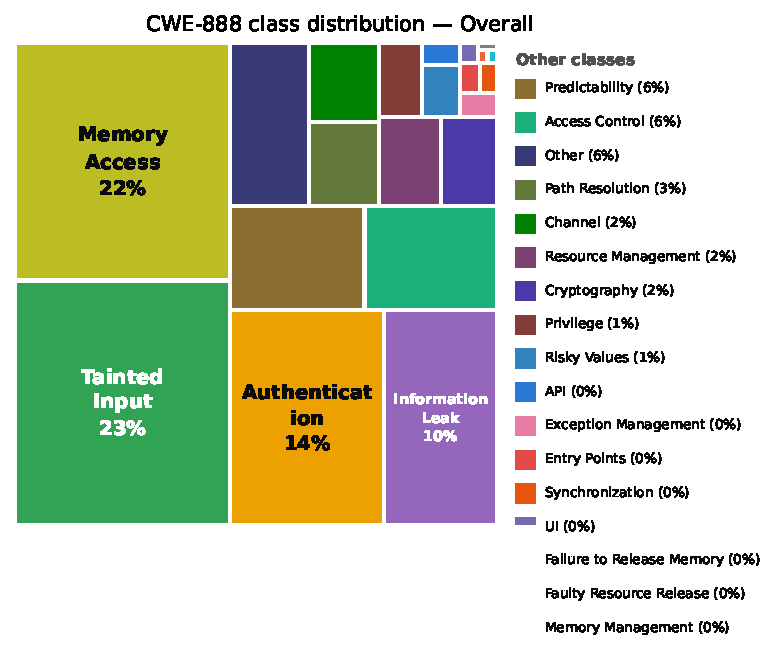
\includegraphics[width=\columnwidth]{figures/cwe888_treemap_all.pdf}
\caption{Distribution of confirmed home IoT CVEs' CWE-888 primary classes, overall.}
\label{fig:cwe888-treemap-all}
\end{figure}

\subsection{Camera vulnerabilities}
\label{sec:rq1-cat1}

Figure~\ref{fig:cwe888-treemap-cameras} shows the distribution of
\texttt{cameras} CWEs across CWE-888 primary classes. The \texttt{cameras}
category is the largest in the study, with 555 confirmed CVEs corresponding to
996 CWE attributions (52\% of the corpus). Its profile is led by
\texttt{Tainted Input} (29\%), followed by \texttt{Memory Access} (17\%),
\texttt{Authentication} (15\%), and \texttt{Information Leak} (10\%). The top
six classes account for 84\% of all camera vulnerabilities (see
Table~\ref{tab:cwe888-matrix}). These devices are network-facing: their
management surface is typically an embedded web interface and their media path
speaks RTSP or ONVIF, exposing externally supplied input to firmware parsers
written in C. Related leaf categories \texttt{doorbell} (21\%
\texttt{Tainted Input}) and \texttt{babymonitor} (18\%) show a similar
profile; together they fold into the Cameras and Monitors group of
Table~\ref{tab:cwe888-family} (28\% \texttt{Tainted Input} overall).

\begin{figure}[t]
\centering
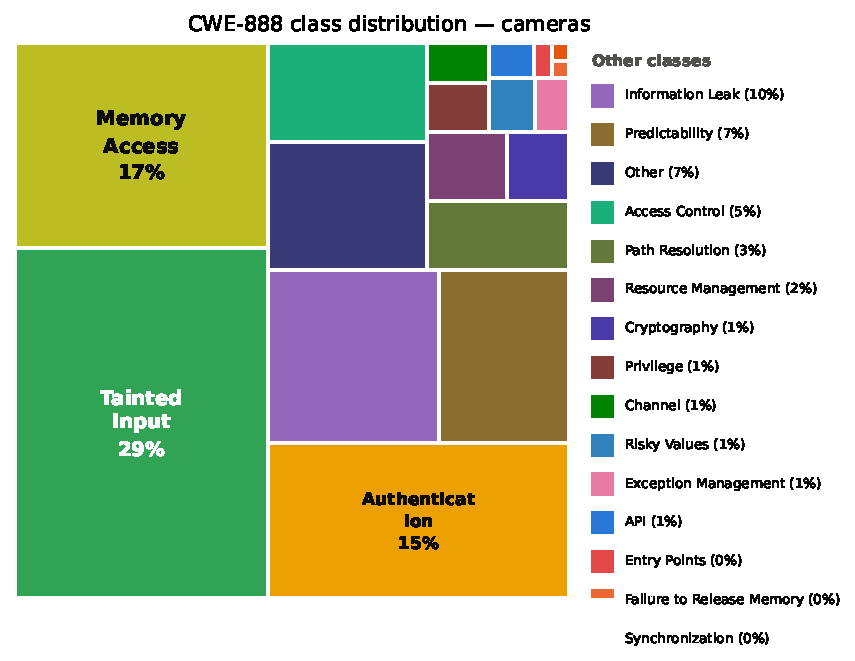
\includegraphics[width=\columnwidth]{figures/cwe888_treemap_cameras.pdf}
\caption{Distribution of \texttt{cameras} category CVEs' CWE-888 primary classes.}
\label{fig:cwe888-treemap-cameras}
\end{figure}

\subsection{Hub vulnerabilities}
\label{sec:rq1-cat2}

Figure~\ref{fig:cwe888-treemap-hub} shows the distribution of \texttt{hub}
CWEs across CWE-888 primary classes. There were 92 confirmed CVEs
corresponding to 282 CWE attributions. The most common class was
\texttt{Memory Access} with 61\% of the CWEs --- the highest share of any class
in any category in this study. The following top six classes made up 91\% of
all hub vulnerabilities: \texttt{Memory Access}, \texttt{Tainted Input},
\texttt{Authentication}, \texttt{Information Leak}, \texttt{Access Control},
and \texttt{Cryptography} (see Table~\ref{tab:cwe888-matrix}). Hubs run the
most substantial software stacks in scope --- full Linux systems bridging
Zigbee, Z-Wave, Thread, and IP --- and memory-safety defects in that native code
are a pivot into every device the hub manages, not merely a compromise of one
endpoint.

\begin{figure}[t]
\centering
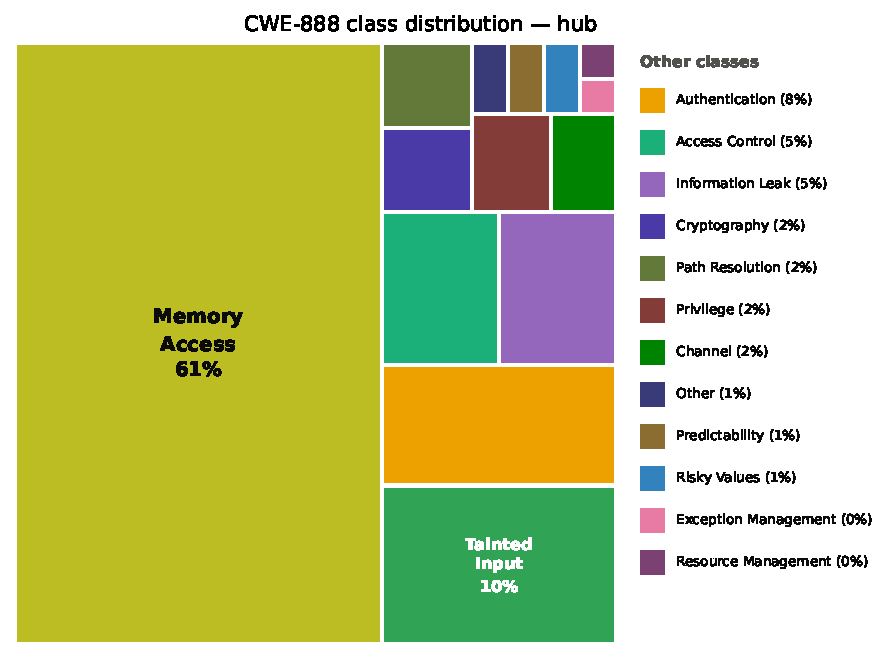
\includegraphics[width=\columnwidth]{figures/cwe888_treemap_hub.pdf}
\caption{Distribution of \texttt{hub} category CVEs' CWE-888 primary classes.}
\label{fig:cwe888-treemap-hub}
\end{figure}

\subsection{Alarm vulnerabilities}
\label{sec:rq1-cat3}

Figure~\ref{fig:cwe888-treemap-alarms} shows the distribution of
\texttt{alarms} CWEs across CWE-888 primary classes. There were 77 confirmed
CVEs corresponding to 86 CWE attributions. The most dominant class was
\texttt{Tainted Input} with 40\% of the CWEs. The top six primary classes
accounted for 90\% of the total vulnerabilities: \texttt{Tainted Input},
\texttt{Information Leak}, \texttt{Channel}, \texttt{Authentication},
\texttt{Predictability}, and \texttt{Access Control}. The elevated
\texttt{Channel} share (14\%) is distinctive: alarm systems rely on wireless
sensor links whose confidentiality and integrity properties have historically
been weak, so a channel-level defect can defeat the system without touching its
application software.

\begin{figure}[t]
\centering
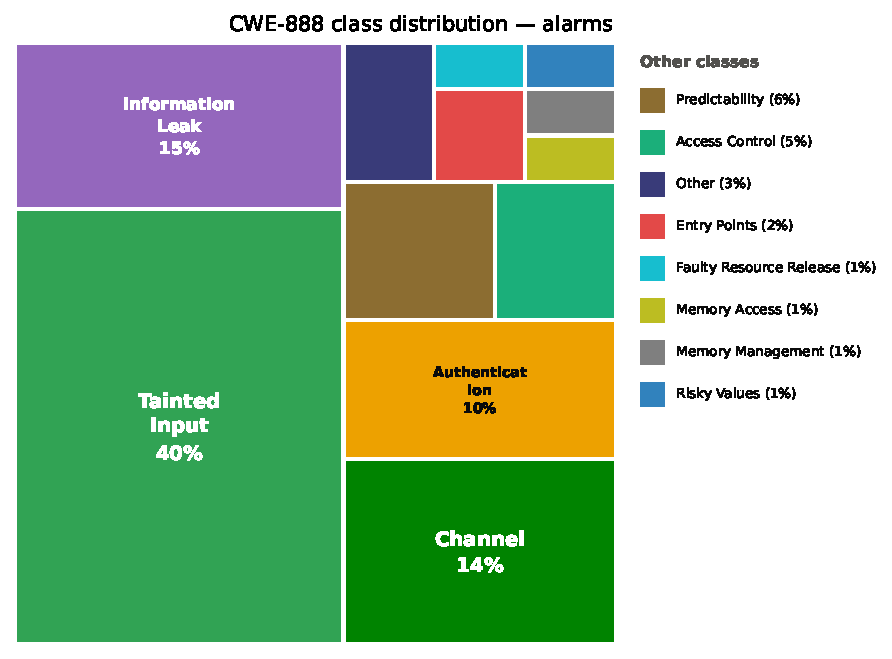
\includegraphics[width=\columnwidth]{figures/cwe888_treemap_alarms.pdf}
\caption{Distribution of \texttt{alarms} category CVEs' CWE-888 primary classes.}
\label{fig:cwe888-treemap-alarms}
\end{figure}

\subsection{EV charging vulnerabilities}
\label{sec:rq1-cat4}

Figure~\ref{fig:cwe888-treemap-evcharging} shows the distribution of
\texttt{ev-charging} CWEs across CWE-888 primary classes. There were 24
confirmed CVEs corresponding to 85 CWE attributions. The profile is more evenly
spread than in cameras or hubs: \texttt{Tainted Input} and \texttt{Memory
Access} each account for 19\%, followed by \texttt{Authentication} (15\%) and
\texttt{Information Leak} (9\%). The top six classes cover 79\% of
attributions. This flatness is consistent with a category spanning
vehicle-charging equipment with OCPP-style backend connectivity, where
authentication and input-validation defects on network-exposed management
interfaces are as prominent as memory-safety issues in embedded firmware.

\begin{figure}[t]
\centering
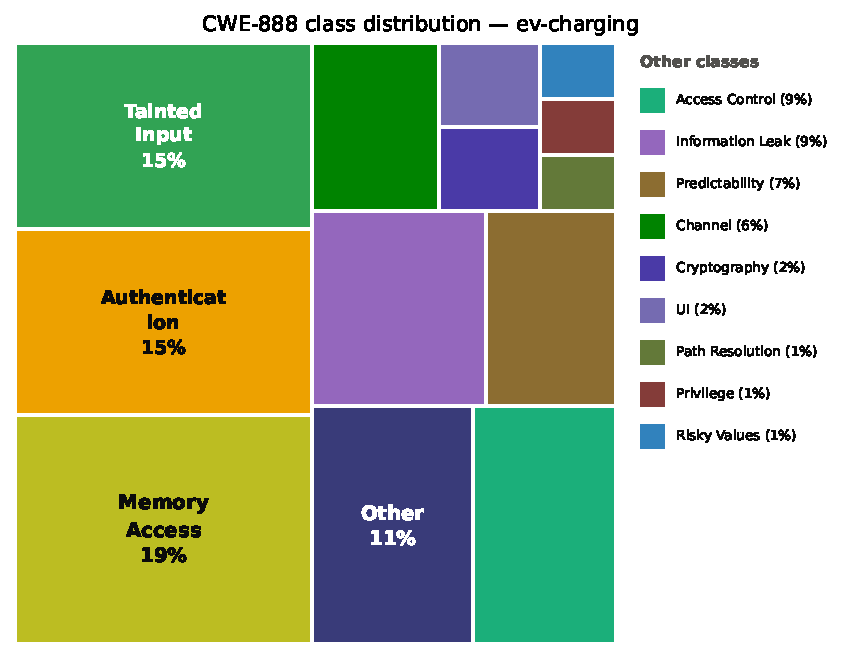
\includegraphics[width=\columnwidth]{figures/cwe888_treemap_ev-charging.pdf}
\caption{Distribution of \texttt{ev-charging} category CVEs' CWE-888 primary classes.}
\label{fig:cwe888-treemap-evcharging}
\end{figure}


%==============================================================================
\section{RQ2: Analysis of CVSS Scores and Severity}
\label{sec:rq2}

In this section we analyze the CVSS scores and severity levels of the confirmed
home IoT device CVEs, summarized in Table~\ref{tab:cvss-summary}. The CVSS score
ranges from 0 to 10 and is a composite metric that integrates the exploitability
and impact of a vulnerability, combined with temporal and environmental
factors~\cite{ref-cvss}. Severity is derived from the score using the standard
qualitative bands described in Section~\ref{sec:method-extract}.

As shown in Table~\ref{tab:cvss-summary}, among the 16 categories with at least
five scored CVEs the highest median CVSS score was found in \texttt{alarms}
(median~8.8, mean~8.21, $n=77$), followed by \texttt{hub} (8.2, 8.09, $n=90$) and
a three-way tie at 8.1 among \texttt{doorlock}, \texttt{home-power}, and
\texttt{garden}. The lowest median was \texttt{babymonitor} (7.2, 6.94, $n=7$),
followed by a tie at 7.4 between \texttt{robotvacuum} and \texttt{pet}. We
conducted a Kruskal-Wallis test across these 16 categories and obtained
$H=77.454$ ($df=15$), $p=2.03\times10^{-10}$, rejecting the null hypothesis that
there is no statistically significant difference among the CVSS scores of the
categories. Four categories --- \texttt{fridge}, \texttt{sensors},
\texttt{appliances}, and \texttt{airconditioner} --- had fewer than five scored
CVEs ($n \le 3$ each) and were excluded from the test; they are reported
descriptively in Table~\ref{tab:cvss-summary} (marked~$\dagger$), but no
statistical conclusion should be drawn from them individually.

The results of Dunn's post-hoc test (rank-based, tie-corrected, two-sided,
Bonferroni-adjusted across all $\binom{16}{2}=120$ pairwise comparisons) showed
that \texttt{streaming} --- by far the largest category by CVE count
($n=2{,}081$) --- had significantly lower CVSS scores than \texttt{alarms}
($p_{\text{bonf}}=6.3\times10^{-6}$), \texttt{hub}
($p_{\text{bonf}}=2.2\times10^{-5}$), and \texttt{cameras}
($p_{\text{bonf}}=4.5\times10^{-3}$). \texttt{alarms} additionally scored
significantly higher than \texttt{robotvacuum} ($p_{\text{bonf}}=0.025$) and
\texttt{cameras} ($p_{\text{bonf}}=0.049$). No other pairs among the 16 tested
categories differed significantly after correction; the full $120$-pair table is
available in the accompanying data release
(Section~\ref{sec:conclusion:data-availability}).

\texttt{alarms} had both the highest mean CVSS score (8.21) among categories with
$n \ge 5$ and the highest critical-severity share of any large category (46.8\%
of its 77 CVEs), consistent with home security/alarm sensors and hubs being
frequent, high-impact targets. \texttt{streaming}, despite dominating the corpus
by CVE count, had a comparatively low critical share (6.4\%) and a majority of
its scores clustered in the High band (55.2\%); \texttt{lighting} showed the
opposite pattern --- the highest concentration in the High band of any category
(62.1\%) but one of the lowest critical shares (6.9\%). \texttt{robotvacuum} and
\texttt{babymonitor} had the lowest mean scores (6.80 and 6.94, respectively),
and neither reported a Critical-severity CVE among its scored CVEs.

Unlike the transportation IoT study, which manually extracted the most
vulnerable \emph{components} (e.g.\ web interface, RKE system, infotainment
system) from each CVE description and cross-tabulated them against severity (its
Table~IV), this study has not yet performed an analogous component-level
extraction. \stub[A component-level breakdown, mirroring Table~IV of the
transportation study, is left as future work (Section~\ref{sec:lessons}) and
would let us test whether specific attack surfaces --- e.g.\ companion mobile
apps, cloud APIs, or physical Zigbee/BLE radio stacks --- concentrate the
Critical/High-severity vulnerabilities the way RKE and web-interface components
did in that study.]

\begin{table*}[t]
\centering
\caption{CVSS score distribution and severity shares for confirmed home IoT
device CVEs, by category. $N$ is the confirmed-\texttt{Yes} CVE count (severity
percentages are of $N$, including any unscored CVEs); Mean/Median/Std are
computed over the subset with a CVSS score. Categories marked $\dagger$ had
$< 5$ scored CVEs and were excluded from the Kruskal-Wallis/Dunn's tests.}
\label{tab:cvss-summary}
\scriptsize
\begin{tabular}{lrrrrrrrr}
\toprule
Category & $N$ & Mean & Median & Std & Critical\% & High\% & Medium\% & Low\% \\
\midrule
doorlock        & 17    & 7.71 & 8.1  & 1.19 & 11.8 & 47.1 & 29.4 & --   \\
smartspeakers   & 31    & 7.46 & 7.6  & 1.88 & 19.4 & 32.3 & 45.2 & 3.2  \\
doorbell        & 23    & 7.86 & 7.5  & 1.44 & 30.4 & 47.8 & 21.7 & --   \\
thermostat      & 8     & 7.94 & 7.85 & 1.82 & 37.5 & 37.5 & 25.0 & --   \\
babymonitor     & 7     & 6.94 & 7.2  & 0.71 & --   & 71.4 & 28.6 & --   \\
smartplugs      & 32    & 7.46 & 7.5  & 1.68 & 21.9 & 37.5 & 40.6 & --   \\
alarms          & 77    & 8.21 & 8.8  & 1.91 & 46.8 & 27.3 & 24.7 & 1.3  \\
robotvacuum     & 23    & 6.80 & 7.4  & 2.05 & 13.0 & 52.2 & 17.4 & 13.0 \\
fridge$\dagger$ & 3     & 7.95 & 7.95 & 2.62 & 33.3 & --   & 33.3 & --   \\
sensors$\dagger$& 2     & 9.10 & 9.1  & 0.00 & 50.0 & --   & --   & --   \\
lighting        & 29    & 7.59 & 7.9  & 1.20 & 6.9  & 62.1 & 31.0 & --   \\
appliances$\dagger$& 3 & 8.13 & 8.1  & 1.65 & 33.3 & 33.3 & 33.3 & --   \\
hub             & 92    & 8.09 & 8.2  & 1.64 & 27.2 & 51.1 & 18.5 & 1.1  \\
ev-charging     & 24    & 7.32 & 7.65 & 1.50 & --   & 58.3 & 41.7 & --   \\
home-power      & 31    & 7.98 & 8.1  & 1.79 & 38.7 & 32.3 & 25.8 & 3.2  \\
garden          & 17    & 7.68 & 8.1  & 2.26 & 35.3 & 35.3 & 17.6 & 11.8 \\
pet             & 29    & 7.12 & 7.4  & 2.25 & 27.6 & 24.1 & 41.4 & 6.9  \\
streaming       & 2{,}081 & 7.25 & 7.8 & 1.56 & 6.4  & 55.2 & 35.9 & 2.5  \\
airconditioner$\dagger$& 1 & 6.30 & 6.3 & 0.00 & --   & --   & 100.0& --   \\
cameras         & 555   & 7.72 & 7.7  & 1.48 & 19.3 & 51.4 & 24.3 & 0.7  \\
\bottomrule
\end{tabular}
\end{table*}

%==============================================================================
\section{Threats to Validity}
\label{sec:threats}

Construct validity relates to the ability to measure what we intend to evaluate.
As in other studies on security vulnerabilities, we searched for information on
NIST's NVD and MITRE's CWE, which are widely used.
\label{sec:threats-construct} Our operationalization of
``home IoT device'' rests on five definitional criteria
(Section~\ref{sec:method-scope}), and those criteria require judgment calls at the
margin. We mitigated this by freezing the category list before large-scale collection
and by pinning a shared scope note per category (\texttt{categories.csv}) that every
reviewer judges against. Encoding the criteria as OWL axioms lets an OWL reasoner
reproduce all 27 published in-scope and out-of-scope rulings as a consistency check.
Mapping individual CWEs onto CWE-888 clusters (Section~\ref{sec:method-cwe888}) is a
second construct threat: parent-resolution can count a CWE toward two primary classes.
We follow the same mapping convention as~\cite{ref-mcsoftware} to keep results
comparable.

Internal validity is based on factors that may affect the independent variables
without the researchers' knowledge.
\label{sec:threats-internal}
The vendor and keyword searches are text-based over CVE descriptions and CPE strings,
so classification errors are possible in either direction. We addressed false positives
with three-AI-plus-human review of every difference-set row and a term-precision pass
that flags low-precision terms for pruning (Section~\ref{sec:method-precision}). We
addressed missed CVEs only partially through CPE expansion
(Section~\ref{sec:method-collect}). The quality of the extracted data depends on NVD and
CWE completeness; as with any empirical vulnerability study, undisclosed and zero-day
vulnerabilities cannot be accounted for. Residual reviewer bias remains possible:
systematic differences among AI reviewers mean that scope notes and human escalation
rules are part of the method, not optional metadata.

Conclusion validity threats impact the ability to draw correct conclusions. The
results are based on an analysis of 1{,}676 distinct confirmed CVEs and 1{,}904 CWE
attributions, which constitute a large sample overall. Analyses per IoT device
category, however, are based on smaller sample sizes (from 2 to 996 CWE attributions),
which poses a threat to per-category conclusions, especially for categories with fewer
than five confirmed CVEs.

External validity is focused on the generalizability.
\label{sec:threats-external}
Our results apply to the types of home IoT devices and categories covered in this
paper. The dataset is bounded by NVD's disclosure and CPE-tagging practices, not by
real-world deployment; a device with no public CVE is invisible to this study. The
snapshot is fixed at 2026-06-25, so the study reports a static ``as-of'' picture. A
device-relevant CVE whose description and CPE strings contain none of our search terms
never enters the dataset unless its product was already confirmed through CPE expansion.
To support reproducibility, all searches run against one fixed NVD snapshot rather than
the live API, and every judgment is persisted in a store keyed by (category, CVE). The
Gemini/Gemma reviewer is the one non-deterministic step; we keep one model fixed per
review pass and record which model produced each judgment.
\label{sec:threats-reliability}

%==============================================================================
\section{Lessons Learned and Implications}
\label{sec:lessons}

Our main findings about vulnerabilities reported for home IoT devices are as
follows.

The considered home IoT devices had vulnerabilities reported across the CWE-888
primary classes, with the top six classes accounting for 81\% of all
attributions corpus-wide. The six most common primary classes together were
\texttt{Tainted Input}, \texttt{Memory Access}, \texttt{Authentication},
\texttt{Information Leak}, \texttt{Access Control}, and \texttt{Other}. This
finding is consistent with~\cite{ref-mcsoftware}, which reported that security
vulnerabilities in mission-critical software were unevenly distributed, with
the top five primary classes contributing from around 80\% to 90\% of
vulnerabilities in each dataset.

In each of the four largest categories discussed in Section~\ref{sec:rq1}, the
six most common primary classes accounted for 79\% to 91\% of all reported
vulnerabilities. For \texttt{cameras}, \texttt{hub}, \texttt{alarms}, and
\texttt{ev-charging}, the top-six shares were 84\%, 91\%, 90\%, and 79\%,
respectively. The most prominent classes differ by architecture, however.
\texttt{cameras} lead with \texttt{Tainted Input} (29\%), reflecting embedded
web interfaces and RTSP/ONVIF parsers; \texttt{hub} with \texttt{Memory Access}
(61\%), reflecting large native-code stacks on Linux controllers;
\texttt{alarms} with \texttt{Tainted Input} (40\%) and an elevated
\texttt{Channel} share (14\%) from wireless sensor links; and \texttt{ev-charging}
with a flatter mix of \texttt{Tainted Input}, \texttt{Memory Access}, and
\texttt{Authentication}. There were similarities but also differences among the
top six dominant vulnerability classes for different IoT device categories.
\texttt{Information Leak} and \texttt{Authentication} appeared among the leading
classes in most large categories, while \texttt{Memory Access} dominated only
the controller-style devices.

Our main findings related to CVSS scores and severity are as follows.
\texttt{alarms} had the highest mean and median CVSS scores and the highest
critical-severity share (46.8\%) among categories with $n \ge 5$.
\texttt{hub} and \texttt{doorlock} also scored at the top of the distribution.
\texttt{cameras}, despite supplying 52\% of CWE attributions, clustered in the
High severity band with a lower critical share (19.3\%). A Kruskal--Wallis test
rejected the null hypothesis of equal CVSS distributions across categories
($p < 10^{-9}$), and Dunn's post-hoc test showed statistically significant
pairwise differences involving \texttt{alarms}, \texttt{hub}, and
\texttt{cameras}.

Our findings have the following actionable implications that could be useful for
developers, manufacturers, and researchers. Focusing on several dominant CWE
classes is an efficient way to improve the security of home IoT devices --- for
example, through secure software development and code-review checklists centered
on input validation, memory safety, authentication, and information disclosure.
Hub and alarm products warrant stricter verification because both weakness
profiles and CVSS scores indicate higher downstream impact when a controller or
security sensor is compromised. Text search over NVD is necessary but
insufficient: 47.8\% of our raw candidates were false positives, so scope
criteria, blind review, and term-list refinement must accompany any NVD-mining
pipeline. Publishing scope notes and search terms alongside mined datasets would
let future studies reproduce and extend our corpus without re-learning the same
false-positive lessons.

%==============================================================================
\section{Conclusions}
\label{sec:conclusion}

This paper is focused on empirical analysis of security vulnerabilities in home
IoT devices. Specifically, we identified the dominant vulnerability classes in
24 categories of home IoT devices and analyzed their CVSS severity scores. Our
results showed that the distribution of vulnerabilities is skewed, with the top
six CWE-888 classes accounting for 81\% of all attributions corpus-wide, and
for 79\% to 91\% within each of the four largest categories. \texttt{alarms}
and \texttt{hub} had the highest CVSS scores among well-populated categories,
with statistically significant differences from several other categories. In
addition to compiling the lessons learned, we identified the implications of our
findings and provided insights that can be used by researchers, developers, and
manufacturers to cost-efficiently improve the security of home IoT devices.

Our future research includes (i)~component-level extraction from CVE
descriptions (web interface, companion app, cloud API, radio stack), mirroring the
transportation IoT study; (ii)~data triangulation with deployment-oriented
sources such as Shodan and Censys; and (iii)~continued refinement of vendor and
keyword term lists in categories where recall estimation indicates thin brand
coverage.

%==============================================================================
\section*{Data Availability}
\label{sec:conclusion:data-availability}

The scripts and derived datasets supporting this study are available at
\stub[repository URL / DOI]. The repository includes: the vendor/brand and keyword term
lists used for collection (\texttt{vendor\_terms.csv}, \texttt{keyword\_terms.csv}); the
raw per-category search outputs (\texttt{results\_all\_<category>.xlsx},
\texttt{keyword\_<category>.csv}); the offline search engine and pipeline scripts (CVE
collection, set reconciliation, CPE expansion, review generation and merging, and
term-precision); the shared classification rubric and per-category scope notes used
by every reviewer (\texttt{CLASSIFICATION\_PROMPT.md}, \texttt{categories.csv}); the
blind per-reviewer judgment files and their merged, human-adjudicated, and finalized outputs
for every category; and the persistent judgment store keyed by (category, CVE) that backs
the entire review process. The device ontology is included as a citable artifact in its own
right: \texttt{homeiot.ttl} (the OWL~2 class hierarchy, criterion facets, and folding
categories), \texttt{shapes.ttl} (the SHACL constraints every class must satisfy),
\texttt{homeiot-align.ttl} (alignment to SAREF and SSN/SOSA, kept in a separate file so it
can be dropped without affecting the pipeline, together with the pinned manifest of
external class IRIs it is validated against), and \texttt{families.csv} (the generated
leaf-to-folding-category map used for the rollups in Section~\ref{sec:rq1}). We also
publish \texttt{homeiot-kg.ttl}, an RDF knowledge graph of the confirmed dataset that
expresses every CVE, product, vendor, category assignment, and CWE-888 class as linked
data, so the counts reported in this paper can be reproduced by SPARQL query rather than
by re-running the pipeline. The one artifact not tracked in the repository is the bulk NVD
snapshot itself (\texttt{nvd\_all.csv}, 360{,}981 CVE records merged from the NVD 2.0
API as of 2026-06-25), which is excluded for size rather than for access reasons; the
snapshot's provenance and exact rebuild procedure are documented in
\texttt{data/nvd-snapshot/SNAPSHOT.md} so that it can be regenerated in full from public NVD
data. \stub[State any additional restrictions, e.g.\ whether the repository is public at
publication time or shared upon request, and whether an API key is required to rebuild the
snapshot (NVD and Gemini/Gemma keys are read from a local, gitignored \texttt{.env} and are
not themselves part of the dataset).]

%==============================================================================
\begin{thebibliography}{00}
\bibitem{ref-nvd} NIST, ``National Vulnerability Database (NVD),''
  \url{https://nvd.nist.gov/}.
\bibitem{ref-mcsoftware} K. Goseva-Popstojanova and J. Tyo, ``Experience report:
  Security vulnerability profiles of mission critical software: Empirical
  analysis of security related bug reports,'' in \emph{IEEE 28th Int. Symp. on
  Software Reliability Engineering (ISSRE)}, 2017, pp.~152--163.
\bibitem{ref-cwe888} Common Weakness Enumeration, ``CWE-888: Software Fault
  Pattern (SFP) Clusters,''
  \url{https://cwe.mitre.org/data/definitions/888.html}.
\bibitem{ref-cwe699} Common Weakness Enumeration, ``CWE-699: Software
  Development,'' \url{https://cwe.mitre.org/data/definitions/699.html}.
\bibitem{ref-cwe} Common Weakness Enumeration, ``CWE,''
  \url{https://cwe.mitre.org/data/index.html}.
\bibitem{ref-cvss} FIRST, ``Common Vulnerability Scoring System (CVSS):
  Specification Document,'' \url{https://www.first.org/cvss/}.

% --- Home IoT definition, scope, taxonomy, and category studies (from meeting doc) ---
\bibitem{balta2013} N. Balta-Ozkan, R. Davidson, M. Bicket, and L. Whitmarsh,
  ``Social barriers to the adoption of smart homes,'' \emph{Energy Policy}, vol.~63,
  pp.~363--374, 2013.
\bibitem{alrawi2019} O. Alrawi, C. Lever, M. Antonakakis, and F. Monrose, ``SoK:
  Security evaluation of home-based IoT deployments,'' in \emph{IEEE Symp. on Security
  and Privacy (S\&P)}, 2019.
\bibitem{bugeja2018} J. Bugeja, P. Davidsson, and A. Jacobsson, ``Functional
  classification and quantitative analysis of smart connected home devices,'' in
  \emph{Global Internet of Things Summit (GIoTS)}, 2018, pp.~1--6.
\bibitem{kumar2019} D. Kumar, J. Sorber, A. Lau, A. C. Snoeren, and N. Feamster, ``All
  things considered: An analysis of IoT devices on home networks,'' in \emph{USENIX
  Security Symposium}, 2019.
\bibitem{fakhrhosseini2025} S. FakhrHosseini, C. Lee, S.-H. Lee, and J. Coughlin, ``A
  taxonomy of home automation: Expert perspectives on the future of smarter homes,''
  \emph{Information Systems Frontiers}, vol.~27, no.~2, pp.~449--466, 2025.
\bibitem{hammi2022} M. T. Hammi \emph{et al.}, ``Survey on smart homes: Vulnerabilities,
  risks, and countermeasures,'' \emph{Computers \& Security}, 2022.
\bibitem{nistir8267} National Institute of Standards and Technology, ``Security review
  of consumer home Internet of Things (IoT) products,'' NIST IR 8267, 2019.
\bibitem{nistir8259a} National Institute of Standards and Technology, ``IoT device
  cybersecurity capability core baseline,'' NIST IR 8259A, 2020.
\bibitem{nistir8425} National Institute of Standards and Technology, ``Profile of the
  IoT core baseline for consumer IoT products,'' NIST IR 8425, 2022.
\bibitem{xenofontos2021} C. Xenofontos \emph{et al.}, ``Consumer, commercial and
  industrial IoT (in)security: Attack taxonomy and case studies,''
  \emph{arXiv:2105.06612}, 2021.
\bibitem{wurm2016} J. Wurm \emph{et al.}, ``Security analysis on consumer and industrial
  IoT devices,'' in \emph{Asia and South Pacific Design Automation Conf. (ASP-DAC)},
  2016, pp.~519--524.
\bibitem{alladi2020} T. Alladi, V. Chamola, B. Sikdar, and K.-K. R. Choo, ``Consumer
  IoT: Security vulnerability case studies and solutions,'' \emph{IEEE Consumer
  Electronics Magazine}, vol.~9, no.~2, pp.~17--25, 2020.
\bibitem{ugwuanyi2021} U. Ugwuanyi and J. Irvine, ``Industrial and consumer internet of
  things: Cyber security considerations, threat landscape, and countermeasure
  opportunities,'' in \emph{SmartNets Conf.}, 2021.
\bibitem{taxonomyci2023} ``Taxonomy of consumer and industrial IoT,'' in \emph{IEEE
  SoutheastCon}, 2023.
\bibitem{stanford_iot} Stanford University, ``Minimum security standards: Internet of
  Things (IoT) devices.'' \url{https://uit.stanford.edu/guide/securitystandards/iot}.
\bibitem{sanders2017} C. Sanders \emph{et al.}, ``Smart secure homes: A survey of smart
  home technologies that sense, assess, and respond to security threats,''
  \emph{Buildings}, vol.~7, no.~3, p.~55, 2017.
\bibitem{apthorpe2019} N. Apthorpe \emph{et al.}, ``Privacy and security in
  internet-connected cameras,'' in \emph{IEEE Int. Conf. on Internet of Things (ICIOT)},
  2019.
\bibitem{albrecht2015} K. Albrecht and L. McIntyre, ``Privacy nightmare: When baby
  monitors go bad,'' \emph{IEEE Technology and Society Magazine}, vol.~34, no.~3,
  pp.~14--19, 2015.
\bibitem{jacobsson2018} A. Jacobsson, ``An investigation of vulnerabilities in smart
  connected cameras,'' in \emph{IEEE PerCom Workshops}, 2018.
\bibitem{fernandes2016} E. Fernandes \emph{et al.}, ``Security analysis of emerging
  smart home applications,'' in \emph{IEEE Symp. on Security and Privacy (S\&P)}, 2016,
  pp.~636--654.
\bibitem{apthorpe2017} N. Apthorpe, D. Reisman, and N. Feamster, ``A smart home is no
  castle: Privacy vulnerabilities of encrypted IoT traffic,'' \emph{arXiv:1705.06805},
  2017.
\bibitem{notra2014} S. Notra, M. Siddiqi, H. Habibi Gharakheili, V. Sivaraman, and R.
  Boreli, ``An experimental study of security and privacy risks with emerging household
  appliances,'' in \emph{M2MSec Workshop}, 2014.
\bibitem{loi2017} F. Loi, A. Sivanathan, H. Habibi Gharakheili, A. Radford, and V.
  Sivaraman, ``Systematically evaluating security and privacy for consumer IoT
  devices,'' in \emph{Workshop on Internet of Things Security and Privacy}, 2017.
\bibitem{davis2020} B. D. Davis, J. C. Mason, and M. Anwar, ``Vulnerability studies and
  security postures of IoT devices: A smart home case study,'' \emph{IEEE Internet of
  Things Journal}, vol.~7, no.~10, pp.~10102--10110, 2020.
\bibitem{alsubaei2018} F. Alsubaei, A. Abuhmed, A. Alzahrani, and A. Alshehri, ``Cyber
  and physical security vulnerability assessment for IoT-based smart homes,''
  \emph{Sensors}, vol.~18, no.~3, p.~817, 2018.
\bibitem{zhou2019} W. Zhou \emph{et al.}, ``Discovering and understanding the security
  hazards in the interactions between IoT devices, mobile apps, and clouds on smart home
  platforms,'' in \emph{USENIX Security Symposium}, 2019.
\bibitem{vetrivel2023} S. Vetrivel \emph{et al.}, ``Examining consumer reviews to
  understand security and privacy issues in the market of smart home devices,'' in
  \emph{USENIX Security Symposium}, 2023.
\bibitem{voicecontrol2022} ``Taxonomic classification of IoT smart home voice control,''
  \emph{arXiv:2210.15656}, 2022.
\bibitem{brooks2022} C. Brooks \emph{et al.}, ``Review of electric vehicle charger
  cybersecurity vulnerabilities, potential impacts, and defenses,'' \emph{Energies},
  vol.~15, no.~11, p.~3931, 2022.
\bibitem{sandia2020} Sandia National Laboratories, ``Recommended cybersecurity practices
  for EV charging systems,'' SAND2020-11401, 2020.
\bibitem{fernandez2023} M. Fernandez \emph{et al.}, ``The digital harms of smart home
  devices: A systematic literature review,'' \emph{Computers in Human Behavior},
  vol.~145, p.~107885, 2023.
\bibitem{sivaraman2019} V. Sivaraman \emph{et al.}, ``Beware of the app! On the
  vulnerability surface of smart devices through their companion apps,''
  \emph{arXiv:1901.10062}, 2019.
\bibitem{neupane2022} S. Neupane \emph{et al.}, ``On the data privacy, security, and risk
  postures of IoT mobile companion apps,'' in \emph{IFIP WG 11.3 Conf. on Data and
  Applications Security and Privacy (DBSec)}, 2022, pp.~162--182.
\bibitem{iotflow2023} ``IoTFlow: Inferring IoT device behavior at scale through static
  mobile companion app analysis,'' in \emph{ACM Conf. on Computer and Communications
  Security (CCS)}, 2023.
\bibitem{antonakakis2017} M. Antonakakis \emph{et al.}, ``Understanding the Mirai
  botnet,'' in \emph{USENIX Security Symposium}, 2017.
\bibitem{zheng2022} Y. Zheng \emph{et al.}, ``A comprehensive survey of security issues
  of smart home system: `Spear' and `Shields,' theory and practice,'' \emph{IEEE
  Access}, 2022.
\bibitem{georgiadou2024} A. Georgiadou \emph{et al.}, ``Review of smart-home security
  using the Internet of Things,'' \emph{Electronics}, vol.~13, no.~16, p.~3343, 2024.
\bibitem{owasp} OWASP Foundation, ``OWASP Internet of Things Project.''
  \url{https://owasp.org/www-project-internet-of-things/}.

% --- Related methodology: NVD-based / AI-assisted CVE characterization (from meeting doc) ---
\bibitem{rezaei2026} A. Rezaei \emph{et al.}, ``SoK: Understanding the state of
  IoT-specific vulnerabilities via CVE characterization with LLIoT,'' 2026.
  \url{https://conand.me/publications/rezaei-lliot-2026.pdf}.
\bibitem{chen2024} X. Chen, Y. Yang, Y. Nan, and Y. Zheng, ``An empirical study of
  high-risk vulnerabilities in IoT systems,'' \emph{IEEE Internet of Things Journal},
  2024. \url{https://doi.org/10.1109/jiot.2024.3506976}.
\bibitem{singla2023} A. Singla, S. Reddy, R. Bettati, and H. Alnuweiri, ``Toward a
  multidimensional analysis of the National Vulnerability Database,'' \emph{IEEE
  Access}, 2023. \url{https://doi.org/10.1109/access.2023.3309850}.
\bibitem{firmrec2024} \stub[verify title/authors] ``FirmRec,'' in \emph{ACM Conf. on
  Computer and Communications Security (CCS)}, 2024.
\end{thebibliography}

\end{document}
